\chapter{Implementierung}
\label{chapter5}
Wie bereits erwähnt erfolgt die Implementierung in Java.
Damit für die Nutzung keine weiteren Installationen nötig sind,
werden nur die Java-Standardbibliotheken zur Umsetzung genutzt.
Der gesamte Source Code kann unter \href{https://github.com/lzfs/tsprocessor}{github.com/lzfs/tsprocessor}
abgerufen werden.
In diesem Kapitel wird vertiefend auf die Struktur des Tools eingegangen.
Zudem werden wichtige Aspekte der Implementierung betrachtet.

\section{Aufbau}
\label{5-Aufbau}
Der detailierte Aufbau des Tools kann dem Klassendiagramm in \autoref{fig:Classes} entnommen werden.
Dabei wurde aus Gründen der Übersichtlichkeit auf Konstruktoren,
Getter- und Setter-Methoden verzichtet.
\begin{figure}[p]
    \begin{center}
        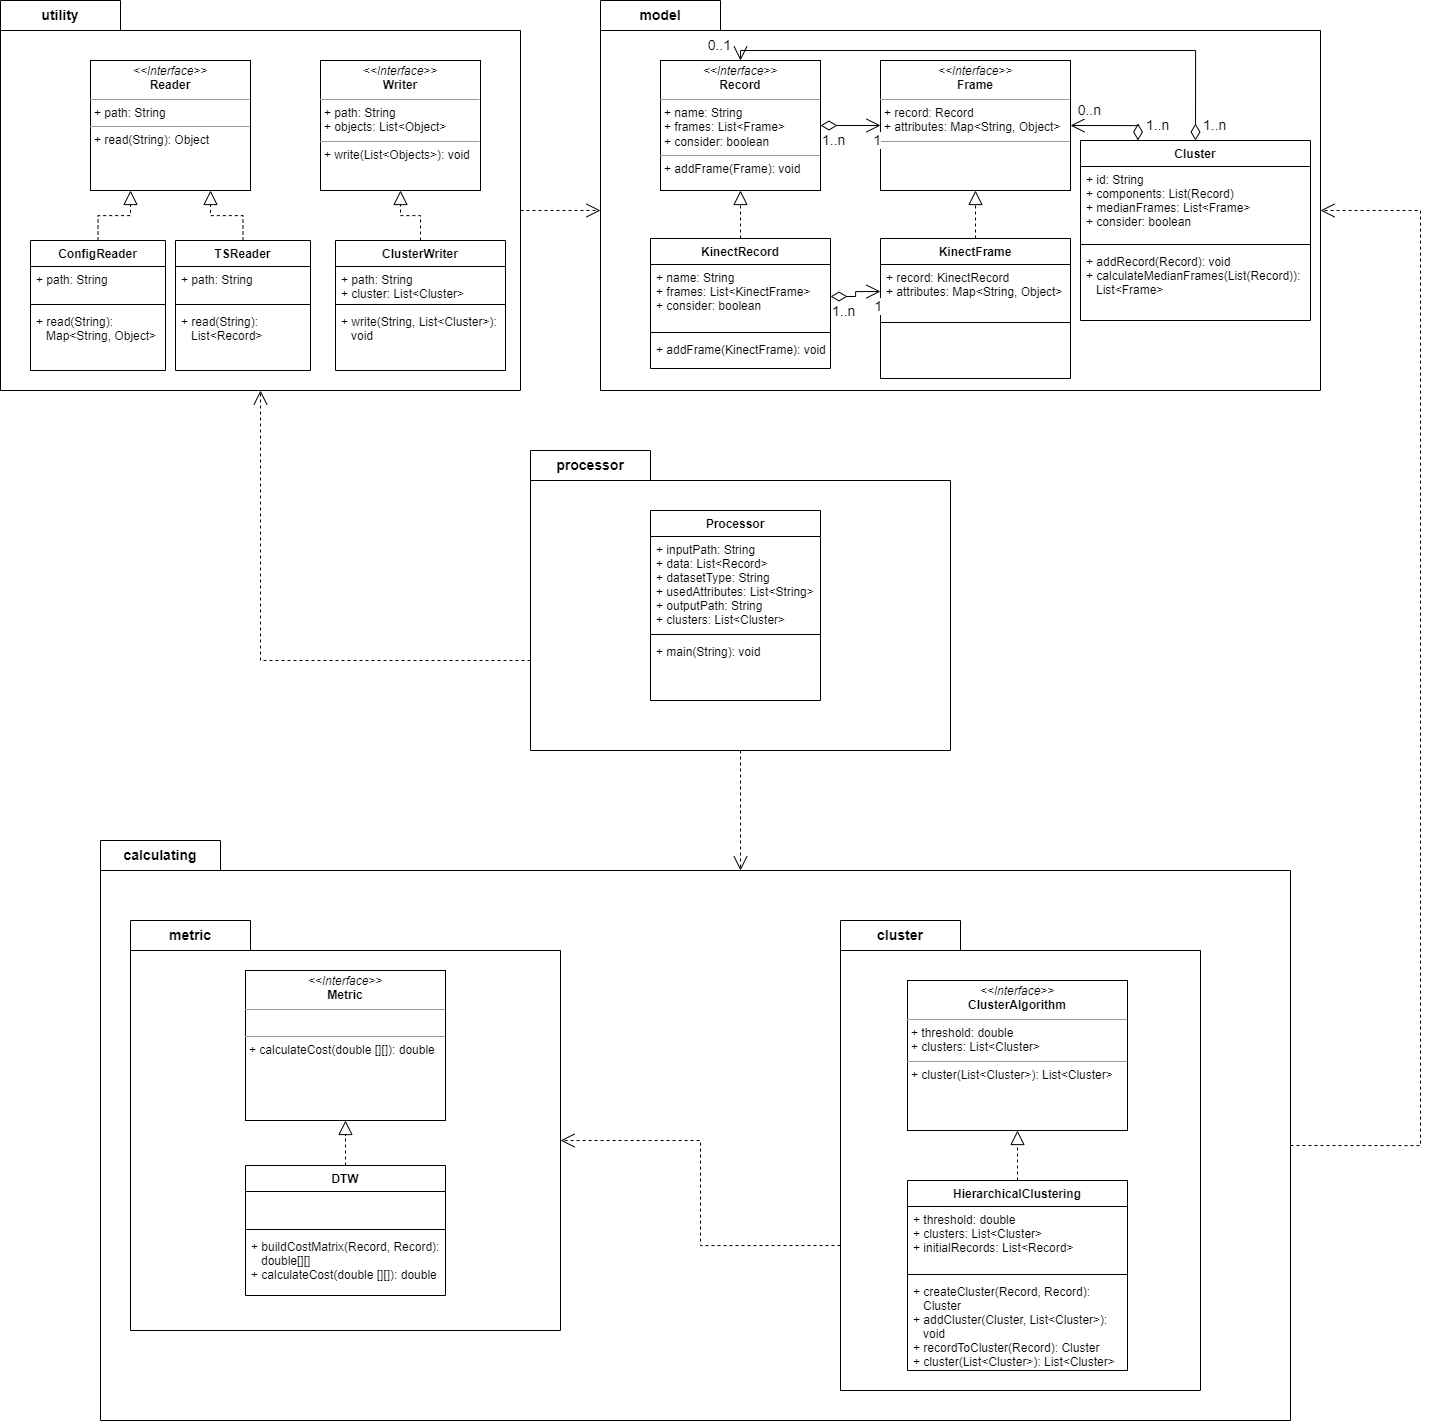
\includegraphics[width=0.6\textwidth]{classes.png}
    \end{center}
    \caption{Klassendiagramm des Tools.}
    \label{fig:Classes}
\end{figure}
Die wichtigsten Aspekte der Software werden im Folgenden beschrieben.
Die grobe Struktur entspricht der aus \autoref{4-Teilsysteme}.
Zum Start der Anwendung ist ein Aufruf der \emph{main-Methode} des \emph{Processor} nötig.
Dieser initialisiert zunächst geeignete \emph{Reader}.
Das \emph{Reader-Interface} wird von den Klassen \emph{ConfigReader} und \emph{DataReader} implementiert.
Der \emph{ConfigReader} dient lediglich dazu die Werte der Config-Datei einzulesen.
Dabei wird ein \emph{Properties-Objekt} zurückgeliefert,
mit dem auf die jeweiligen Werte zugegriffen werden kann.
Der \emph{DataReader} liest die Kinect-Daten ein.
Ihm wird zunächst übermittelt, welche Attribute vorhanden sind,
durch welches Zeichen sie voneinander abgetrennt sind
und ob \emph{Frames} übersprungen werden sollen,
um die Performanz zu verbessern.
Mit diesen Informationen können die Daten geeignet eingelesen und eine \emph{RecordImpl-Liste} zurückgeliefert werden.
Jede \emph{RecordImpl} enthält dabei eine Liste von \emph{FrameImpl}.
Diese Datentypen sind die entsprechenden Implementierungen der Interfaces \emph{Record} und \emph{Frame}.
Sie können für Kinect-Daten genutzt werden.
Eine \emph{FrameImpl} enthält jeweils eine Map mit ihren Attributen.
Diese können mithilfe der \emph{getValue-Methode} abgerufen werden.
Ein weiterer Datentyp ist das \emph{Cluster} und die zugehörige \emph{ClusterImpl}.
Cluster bestehen aus beliebig vielen, aber mindestens einer \emph{RecordImpl}.
Die Bestandteile werden in einer Liste gespeichert.
Hier werden die Methoden \emph{mergeWithCluster} und \emph{mergeWithRecord} angeboten.
Mit ihnen wird jeweils eine weitere Komponente in die \emph{ClusterImpl} integriert.
\emph{ClusterImpls} haben außerdem eine eindeutige Identifikationsnummer und eine Liste der berechneten
\emph{FrameImpl-Mittelwerte} aller Komponenten.
Zudem besitzen sie, genau wie die \emph{RecordImpls}, einen Wahrheitswert der angibt,
ob die \emph{ClusterImpl} in zukünftigen Kombinationsschritten weiterhin beachtet werden soll.
Alle genannten Interfaces können bei Bedarf geeignet für andere \ac{TSD}-Datensätze implementiert werden.
Nach dem Einlesen und Abspeichern der Daten startet der \emph{Processor} das Clustering.
Dazu wird eine Instanz von \emph{HierarchicalClustering}, einer Implementierung von \emph{ClusterAlgorithm}, erstellt.
Das Objekt erhält dafür alle wichtigen Informationen,
wie die initialen \emph{RecordImpls}, den Threshold und die Attribute vom \emph{Processor}.
Da jede \emph{ClusterImpl} am Anfang aus einer einzigen \emph{RecordImpl} besteht,
wird eine \emph{recordToCluster-Methode} angeboten.
Mit ihr kann jeder der initialen \emph{RecordImpls} transformiert
und anschließend in der \emph{clusterImpl-Liste} abgelegt werden.
Die \emph{cluster-Methode} kümmert sich um den eigentlichen Cluster-Vorgang.
Dabei nutzt sie zur Berechnung von Kosten eine Instanz der \emph{Dtw-Klasse}.
Sie implementiert das \emph{Metric-Interface} und bietet daher die nötigen Methoden,
um die Kosten zwischen zwei \emph{RecordImpls}, beziehungsweise deren \emph{FrameImpl-Listen} zu berechnen.
Dabei kommt der in \autoref{3-DTW} beschriebene \ac{DTW}-Algorithmus zum Einsatz.
Um auch eine \emph{ClusterImpl} mit einer \emph{RecordImpls} vergleichen zu können bietet die Klasse zudem entsprechende
\emph{calculateMedianFrames-Methoden}, die aus mehreren \emph{FrameImpl-Listen} eine neue erzeugt,
indem die Werte mithilfe von \ac{DTW} kombiniert werden.
Das genaue Verhalten der Klassen \emph{HierarchicalClustering} und \emph{Dtw} wird in \autoref{5-Codebeschreibung} näher betrachtet.
Nach dem Ende der Berechnungen liegen die gefundenen \emph{ClusterImpls} in der \emph{clusterImpl-Liste} vor.
Sie werden mit dem \emph{ClusterWriter} geeignet in einer Textdatei abgespeichert.
Zudem kann eine Visualiserung mithilfe der \emph{VisualizerImpl} erfolgen.
Die Klasse nutzt dazu einfache Java-AWT-Komponenten.
Der Wahrheitswert \emph{flipVisualization} gibt dabei an,
ob die Werte in x-Richtung gespiegelt werden sollen.
Dies ist nötig, da bei der Kinect das Koordinatensystem aus Nutzersicht erstellt wird.
In der Visualiserung führt dies dazu, dass die aufgezeichneten Bewegungen spiegelverkehrt erscheinen.
Der String \emph{attributeForBodyIdentification} dient dazu,
die unterschiedlichen Personen im \emph{Record} korrekt darzustellen.

\section{Codebeschreibung}
\label{5-Codebeschreibung}
Nach der Beschreibung des Ablaufs und der groben Struktur
sollen nun wichtige Codeausschnitte des hierarchischen Clusterings
und des \ac{DTW}-Algorithmus beschrieben werden.

Objekte der Klassen ClusterImpl, RecordImpl und FrameImpl werden in diesem Abschnitt
vereinfacht als Cluster, Record und Frame bezeichnet.
Bei der Ausführung des Folgenden Codes wurden die Daten bereits eingelesen.
Zudem wurde ein HierarchicalClustering-Objekt mit den nötigen Parametern erzeugt.
Damit wird die cluster-Methode gestartet.
Die Klasse HierarchicalClustering verfügt über eine clusterImpl-Liste,
welche zunächst leer ist.
Sie wird mit den initialen Clustern belegt,
indem alle Records zunächst zu trivialen Clustern transformiert werden
und anschließend der Liste hinzugefügt werden.
Des Weiteren werden die nötigen Variablen für die Berechnung deklariert.
\begin{lstlisting}[language=Java, caption=Cluster-Methode: Initialisierung.]
  // Initialize each record as a cluster and add it to the clusters list.
  for (RecordImpl record : this.initialRecords) {
      this.clusterImpls.add(this.recordToCluster(record));
  }
  double currentMinimumCost;
  double cost;
  int mergeCandidate1;
  int mergeCandidate2;
\end{lstlisting}
Der eigentliche Berechnungsablauf befindet sich in einer Schleife die mindestens einmal ausgeführt wird.
Sie läuft weiter, bis die geringsten gefundenen Kosten den Threshold übersteigen,
oder nur noch ein einziges Cluster übrig ist.
Die Merge-Kandidaten geben die Indizes der beiden Cluster mit den
geringsten Kombinationskosten an.
In jedem Durchlauf der while-Schleife werden die Werte der Kosten
und die gewählten Merge-Kandidaten zurückgesetzt.
Dazu werden standardmäßig das erste und zweite Cluster in der Liste und deren Kosten gewählt.
Dann werden mittels der geschachtelten Schleifen paarweise die Cluster miteinander verglichen.
Dabei werden nur Cluster in Betracht gezogen deren \emph{consider-Wert} noch \emph{true} ist.
Außerdem darf es sich nicht zweimal um das gleiche Cluster handeln.
Mithilfe der \emph{calculatedCost-Map} wird geprüft, ob die Kosten für diese Kombination schon berechnet wurden.
Falls ja werden sie wieder genutzt, falls nein werden sie neu berechnet.
Als Schlüssel dienst ein Objekt der bereits erwähnten \emph{ClusterKey-Klasse}.
Deren \emph{equal-Methode} ist so definiert,
dass \emph{new ClusterKey(clusterImpl1, clusterImpl2).equals(new ClusterKey(clusterImpl2, clusterImpl1)) == true} gilt.
Somit wird auch der symmetrische Fall betrachtet.
Immer wenn eine Kombination gefunden wird, deren Kosten geringer sind als die bisherigen,
werden die aktuellen Minimalkosten und die Merge-Kandidaten angepasst.
Nach dem Vergleich aller Cluster, erfolgt die Kombination der beiden mit den geringsten Kombinationskosten.
\begin{lstlisting}[language=Java, caption=Cluster-Methode: Berechnungsvorgang.]
  do {
      // Reset for next loop iteration.
      cost = this.dtw.calculateCost(    
          this.clusterImpls.get(0).getMedianFrames(),
          this.clusterImpls.get(1).getMedianFrames());
      currentMinimumCost = cost;
      mergeCandidate1 = 0;
      mergeCandidate2 = 1;
      for (ClusterImpl clusterImpl1 : this.clusterImpls) {
          for (ClusterImpl clusterImpl2 : this.clusterImpls) {
              if (
                  clusterImpl1 != clusterImpl2
                  && clusterImpl1.isConsider()
                  && clusterImpl2.isConsider()) {
                  if (this.calculatedCost.containsKey(
                      new ClusterKey(clusterImpl1, clusterImpl2))) {
                      cost = this.calculatedCost.get(
                          new ClusterKey(clusterImpl1, clusterImpl2));
                  }
                  else {
                      cost = this.dtw.calculateCost(
                          clusterImpl1.getMedianFrames(),
                          clusterImpl2.getMedianFrames());
                      this.calculatedCost.put(
                          new ClusterKey(clusterImpl1, clusterImpl2), cost);
                  }
                  if (cost < currentMinimumCost) {
                      /* If a cost smaller than the current minimum cost
                      has been found it will be the new minimum. */
                      currentMinimumCost = cost;
                      mergeCandidate1 = this.clusterImpls.indexOf(clusterImpl1);
                      mergeCandidate2 = this.clusterImpls.indexOf(clusterImpl2);
                  }
              }
          }
      }
      // Merging. Showed in next Listing.
      } while (currentMinimumCost < threshold && this.clusterImpls.size() > 1);
\end{lstlisting}
Nun wurden die beiden Cluster mit den geringsten Kombinationskosten gefunden.
Die zugehörigen Kosten sind in der Variablen \emph{currentMinimumCost} abgelegt.
Sind diese immer noch geringer als der definierte Threshold können die Kandidaten zusammengeführt werden.
Dazu wird \emph{mergeCandidate2} mit der Methode \emph{mergeWithCluster} in \emph{mergeCandidate1} integriert.
Dabei wird der \emph{consider}-Wert des \emph{mergeCandidate2}-Clusters auf \emph{false} gesetzt,
da es in künftigen Schritten nicht mehr als eigenständige Einheit betrachtet werden soll.
Abschließend müssen alle berechneten Werte mit \emph{cluster1} aus der \emph{calculateCost-Map} entfernt werden,
da die aktuellen Werte aufgrund der neuen Komponente nicht mehr gültig sind.
Die Kosten mit \emph{cluster2} können ignoriert werden, da diese Cluster ohnehin nicht mehr betrachtet werden.
\begin{lstlisting}[language=Java, caption=Cluster-Methode: Mergevorgang.]
  if (currentMinimumCost < threshold) {
      /* MergeCandidate1 and mergeCandidate2 should be merged together.
      Merge cluster2 into cluster1 and update the cluster list.
      Consider of cluster2 is set to false. */
      this.clusterImpls.get(mergeCandidate1).mergeWithCluster(
          this.clusterImpls.get(mergeCandidate2));  
      this.clusterImpls.remove(this.clusterImpls.get(mergeCandidate2));
      // Create a copy of the map to avoid an exception.
      Map<ClusterKey, Double> calculatedCostCopy = new HashMap<>(calculatedCost); 
      /* remove all calculated costs from the map that contain
      cluster1 because it changed and therefore all cost values
      with this cluster have to be calculated again. */
      for (Map.Entry<ClusterKey, Double> entry : calculatedCostCopy.entrySet()) {
          /* Ignore mergeCandidate2 because it got removed from the list and
          the consider value of cluster2 is set to false. */
          if (  entry.getKey().getCluster1().getId() == mergeCandidate1
                || entry.getKey().getCluster2().getId() == mergeCandidate1) {
              for (ClusterImpl clusterImpl : clusterImpls) {
                  calculatedCost.remove(
                      new ClusterKey(
                          this.clusterImpls.get(mergeCandidate1), clusterImpl));
              }
          }
      }
  }
\end{lstlisting}
In den oben gezeigten Clustering-Schritten wurden die Kosten mithilfe der \emph{calculateCost-Methode} berechnet.
Diese wird nun vorgestellt.
Für jedes der Attribute das für die Berechnung verwendet werden soll wird gemäß des \ac{DTW}-Algorithmus
eine Kostenmatrix aufgestellt.
Für sie werden die minimalen Pfadkosten berechnet und zu den Gesamtkosten für diesen Attributvergleich addiert.
Das Ergebnis wird am Ende durch die Anzahl der betrachteten Attribute geteilt,
um auch vergleichbare Werte zu erhalten, wenn die Anzahl an Attributen variiert.
\begin{lstlisting}[language=Java, caption=DTW: Berechnung der Kosten.]
  public double calculateCost(
      List<FrameImpl> frames1,
      List<FrameImpl> frames2) {
      // Add the calculated cost of each attribute to it.
      double cost = 0;
      // calculate the cost for all attributes
      for (String attribute : this.usedAttributes) {
          // Build the cost matrix for this attribute.
          double[][] dtwMatrix = buildCostMatrix(frames1, frames2, attribute);
          // Calculate and add the cost of this attribute.
          cost += calculatePathCost(dtwMatrix);
      }
      return cost / this.usedAttributes.size();
  }
\end{lstlisting}
Die Methode \emph{buildCostMatri}x liefert die passende Kostenmatrix für ein gemeinsames Attribut
zweier Frame-Listen gemäß des \ac{DTW}-Algorithmus.
Zunächst werden die beiden Attributreihen in Arrays kopiert.
Anschließend wird die initiale Matrix erstellt.
Die Zellen der Reihe und Spalte mit dem Index \emph{0} werden mit dem Wert {\glqq unendlich\grqq} belegt.
Die Zelle \emph{(0, 0)} und alle übrigen Zellen erhalten den Wert 0.
Nun werden die Attributwerte paarweise verglichen.
Hier wird standardmäßig die absolute Distanz verwendet.
Bei Bedarf können an dieser Stelle weitere Distanzmetriken ergänzt werden.
Zur berechneten Differenz wird jeweils das Minimum der angrenzenden, bereits berechneten Zellen addiert.
Diese Summe wird in die entsprechende Matrixzelle eingetragen.
Dadurch füllt sich die Matrix und kann nach Abschluss der Berechnungen zurückgegeben werden.
\begin{lstlisting}[language=Java, caption=DTW: Kostenmatrix.]
  private double[][] buildCostMatrix(
      List<FrameImpl> frames1,
      List<FrameImpl> frames2,
      String attribute) {
      double[] s = new double[frames1.size()];
      double[] t = new double[frames2.size()];

      int counter = 0;
      for (FrameImpl frame : frames1) {
          s[counter] = Double.parseDouble(frame.getValue(attribute));
          counter += 1;
      }
      counter = 0;
      for (FrameImpl frame : frames2) {
          t[counter] = Double.parseDouble(frame.getValue(attribute));
          counter += 1;
      }

      int n = s.length;
      int m = t.length;
      // Filled with zeros by default.
      double[][] dtwMatrix = new double[n + 1][m + 1];

      for (int i = 0; i < dtwMatrix.length; i++) {
          for (int j = 0; j < dtwMatrix[0].length; j++) {
              // filled with infinity by definition of dtw
              dtwMatrix[i][j] = Double.POSITIVE_INFINITY;
          }
      }
      // Filled with zero by definition of dtw.
      dtwMatrix[0][0] = 0;

      for (int i = 1; i < dtwMatrix.length; i++) {
          for (int j = 1; j < dtwMatrix[0].length; j++) {
              // this is the default distance function
              double cost = Math.abs(s[i - 1] - t[j - 1]);
              
              double minTmp = Math.min(dtwMatrix[i - 1][j], dtwMatrix[i][j - 1]);
              double lastMin = Math.min(minTmp, dtwMatrix[i - 1][j - 1]);
              dtwMatrix[i][j] = cost + lastMin;
          }
      }
      return dtwMatrix;
  }
\end{lstlisting}
Die Kosten des Warping Pfads der entsprechenden Matrix können mithilfe der Methode \emph{calculatePathCost}
berechnet werden.
Das Verfahren startet in der letzten Zelle der Matrix und sucht den Pfad mit den geringsten Kosten,
um die Zelle \emph{(0, 0)} zu erreichen.
Dabei werden die in \autoref{3-DTW} beschriebenen Vorgaben eingehalten.
Die Kosten des Pfades werden aufsummiert und anschließend durch die Anzahl der betretenen Zellen geteilt.
Diese Division ist nötig, um im Falle von unterschiedlich großen Matrizen vergleichbare Ergebnisse zu erhalten.
\begin{lstlisting}[language=Java, caption=DTW: Warping Path berechnen.]
  public double calculatePathCost(double[][] dtwMatrix) {
      int n = dtwMatrix.length - 1;
      int m = dtwMatrix[n - 1].length - 1;
      int pathCounter = 1;
      double cost = dtwMatrix[n][m];
      while (n != 0 && m != 0) {
          // dynamic time warping algorithm
          double minTmp = Math.min(dtwMatrix[n - 1][m], dtwMatrix[n][m - 1]);
          double lastMin = Math.min(minTmp, dtwMatrix[n - 1][m - 1]);
          cost += lastMin;
          if (lastMin == dtwMatrix[n - 1][m - 1]) {
              n = n - 1;
              m = m - 1;
          }
          else if (lastMin == dtwMatrix[n - 1][m]) {
              n = n - 1;
          }
          else if (lastMin == dtwMatrix[n][m - 1]) {
              m = m - 1;
          }
          pathCounter += 1;
      }
      return cost / pathCounter;
  }
\end{lstlisting}

\section{Abweichungen zur Konzeption}
\label{5-AbweichungenKonzeption}
An die Performanz der Anwendung wurden keine besonderen Anforderungen gestellt
(\autoref{4-NichtFunktionaleAnforderungen}).
Es zeigte sich aber schnell, dass bereits Datensätze mit einigen Hundert Records zu langen Bearbeitungszeiten führen.
Daher wurden zwei Konzepte umgesetzt die sich diesem Problem annehmen.
Zum einen werden die berechneten Kosten in einer Map abgespeichert,
um wiederholte Berechnungen in darauffolgenden Schritten zu vermeiden.
Als Key der jeweiligen Map-Einträge dient ein Objekt der Klasse ClusterKey.
Sie implementiert das Comparable-Interface und sorgt dafür,
dass zwei Cluster zusammen als Key einer Map verwendet werden können.
Dies spart viele Berechnungsschritte,
da beinahe alle Werte im Vergleich zum vorherigen Iterationsschritt gleich bleiben.
Lediglich jene Kosten an denen die neu zusammengeführten Cluster beteiligt waren,
sowie die Kosten mit dem neuen Cluster müssen neu berechnet werden.
Zum anderen gibt es die Möglichkeit jeden dritten Frame der Records zu ignorieren.
Dies geschieht, indem der Parameter \emph{skipFrames} in der config-Datei auf \emph{true} gesetzt wird.
Damit ist in der Regel weiterhin ein sinnvolles Clustering möglich,
wobei die Anzahl der Berechnungsschritte reduziert werden kann.
Es ist zu erwähnen, dass es dabei zu einem Informationsverlust kommt.
Diese Option sollte daher nur bei Bedarf genutzt werden.

Zudem wurde abweichend zur Konzeption ein primitiver \emph{Visualizer} ergänzt,
da sonst die Analyse der Cluster manuell über Kinect Studio erfolgen muss.
Er stellt die Laufwege der gefundenen Cluster aus der Vogelperspektive dar.
Für jedes Cluster wird ein Verzeichnis erstellt.
Darin werden die einzelnen Komponenten visualisiert.